% Created 2021-04-08 qui 18:01
% Intended LaTeX compiler: pdflatex
\documentclass[11pt]{article}
\usepackage[utf8]{inputenc}
\usepackage{lmodern}
\usepackage[T1]{fontenc}
\usepackage[top=3cm, bottom=2cm, left=3cm, right=2cm]{geometry}
\usepackage{graphicx}
\usepackage{longtable}
\usepackage{float}
\usepackage{wrapfig}
\usepackage{rotating}
\usepackage[normalem]{ulem}
\usepackage{amsmath}
\usepackage{textcomp}
\usepackage{marvosym}
\usepackage{wasysym}
\usepackage{amssymb}
\usepackage{amsmath}
\usepackage[theorems, skins]{tcolorbox}
\usepackage[style=abnt,noslsn,extrayear,uniquename=init,giveninits,justify,sccite,
scbib,repeattitles,doi=false,isbn=false,url=false,maxcitenames=2,
natbib=true,backend=biber]{biblatex}
\usepackage{url}
\usepackage[cache=false]{minted}
\usepackage[linktocpage,pdfstartview=FitH,colorlinks,
linkcolor=blue,anchorcolor=blue,
citecolor=blue,filecolor=blue,menucolor=blue,urlcolor=blue]{hyperref}
\usepackage{attachfile}
\usepackage{setspace}
\usepackage{tikz}
\author{Gabriel Petrini}
\date{\today}
\title{Apêndice estatístico (gráficos)}
\begin{document}

\maketitle

\section*{Gráficos adicionais}
\label{sec:orgba1b3c3}

\begin{figure}[htbp]
\caption{Novos casos e mortes a cada 1 milhão de habitantes (Brasil, semana móvel)}
\centering
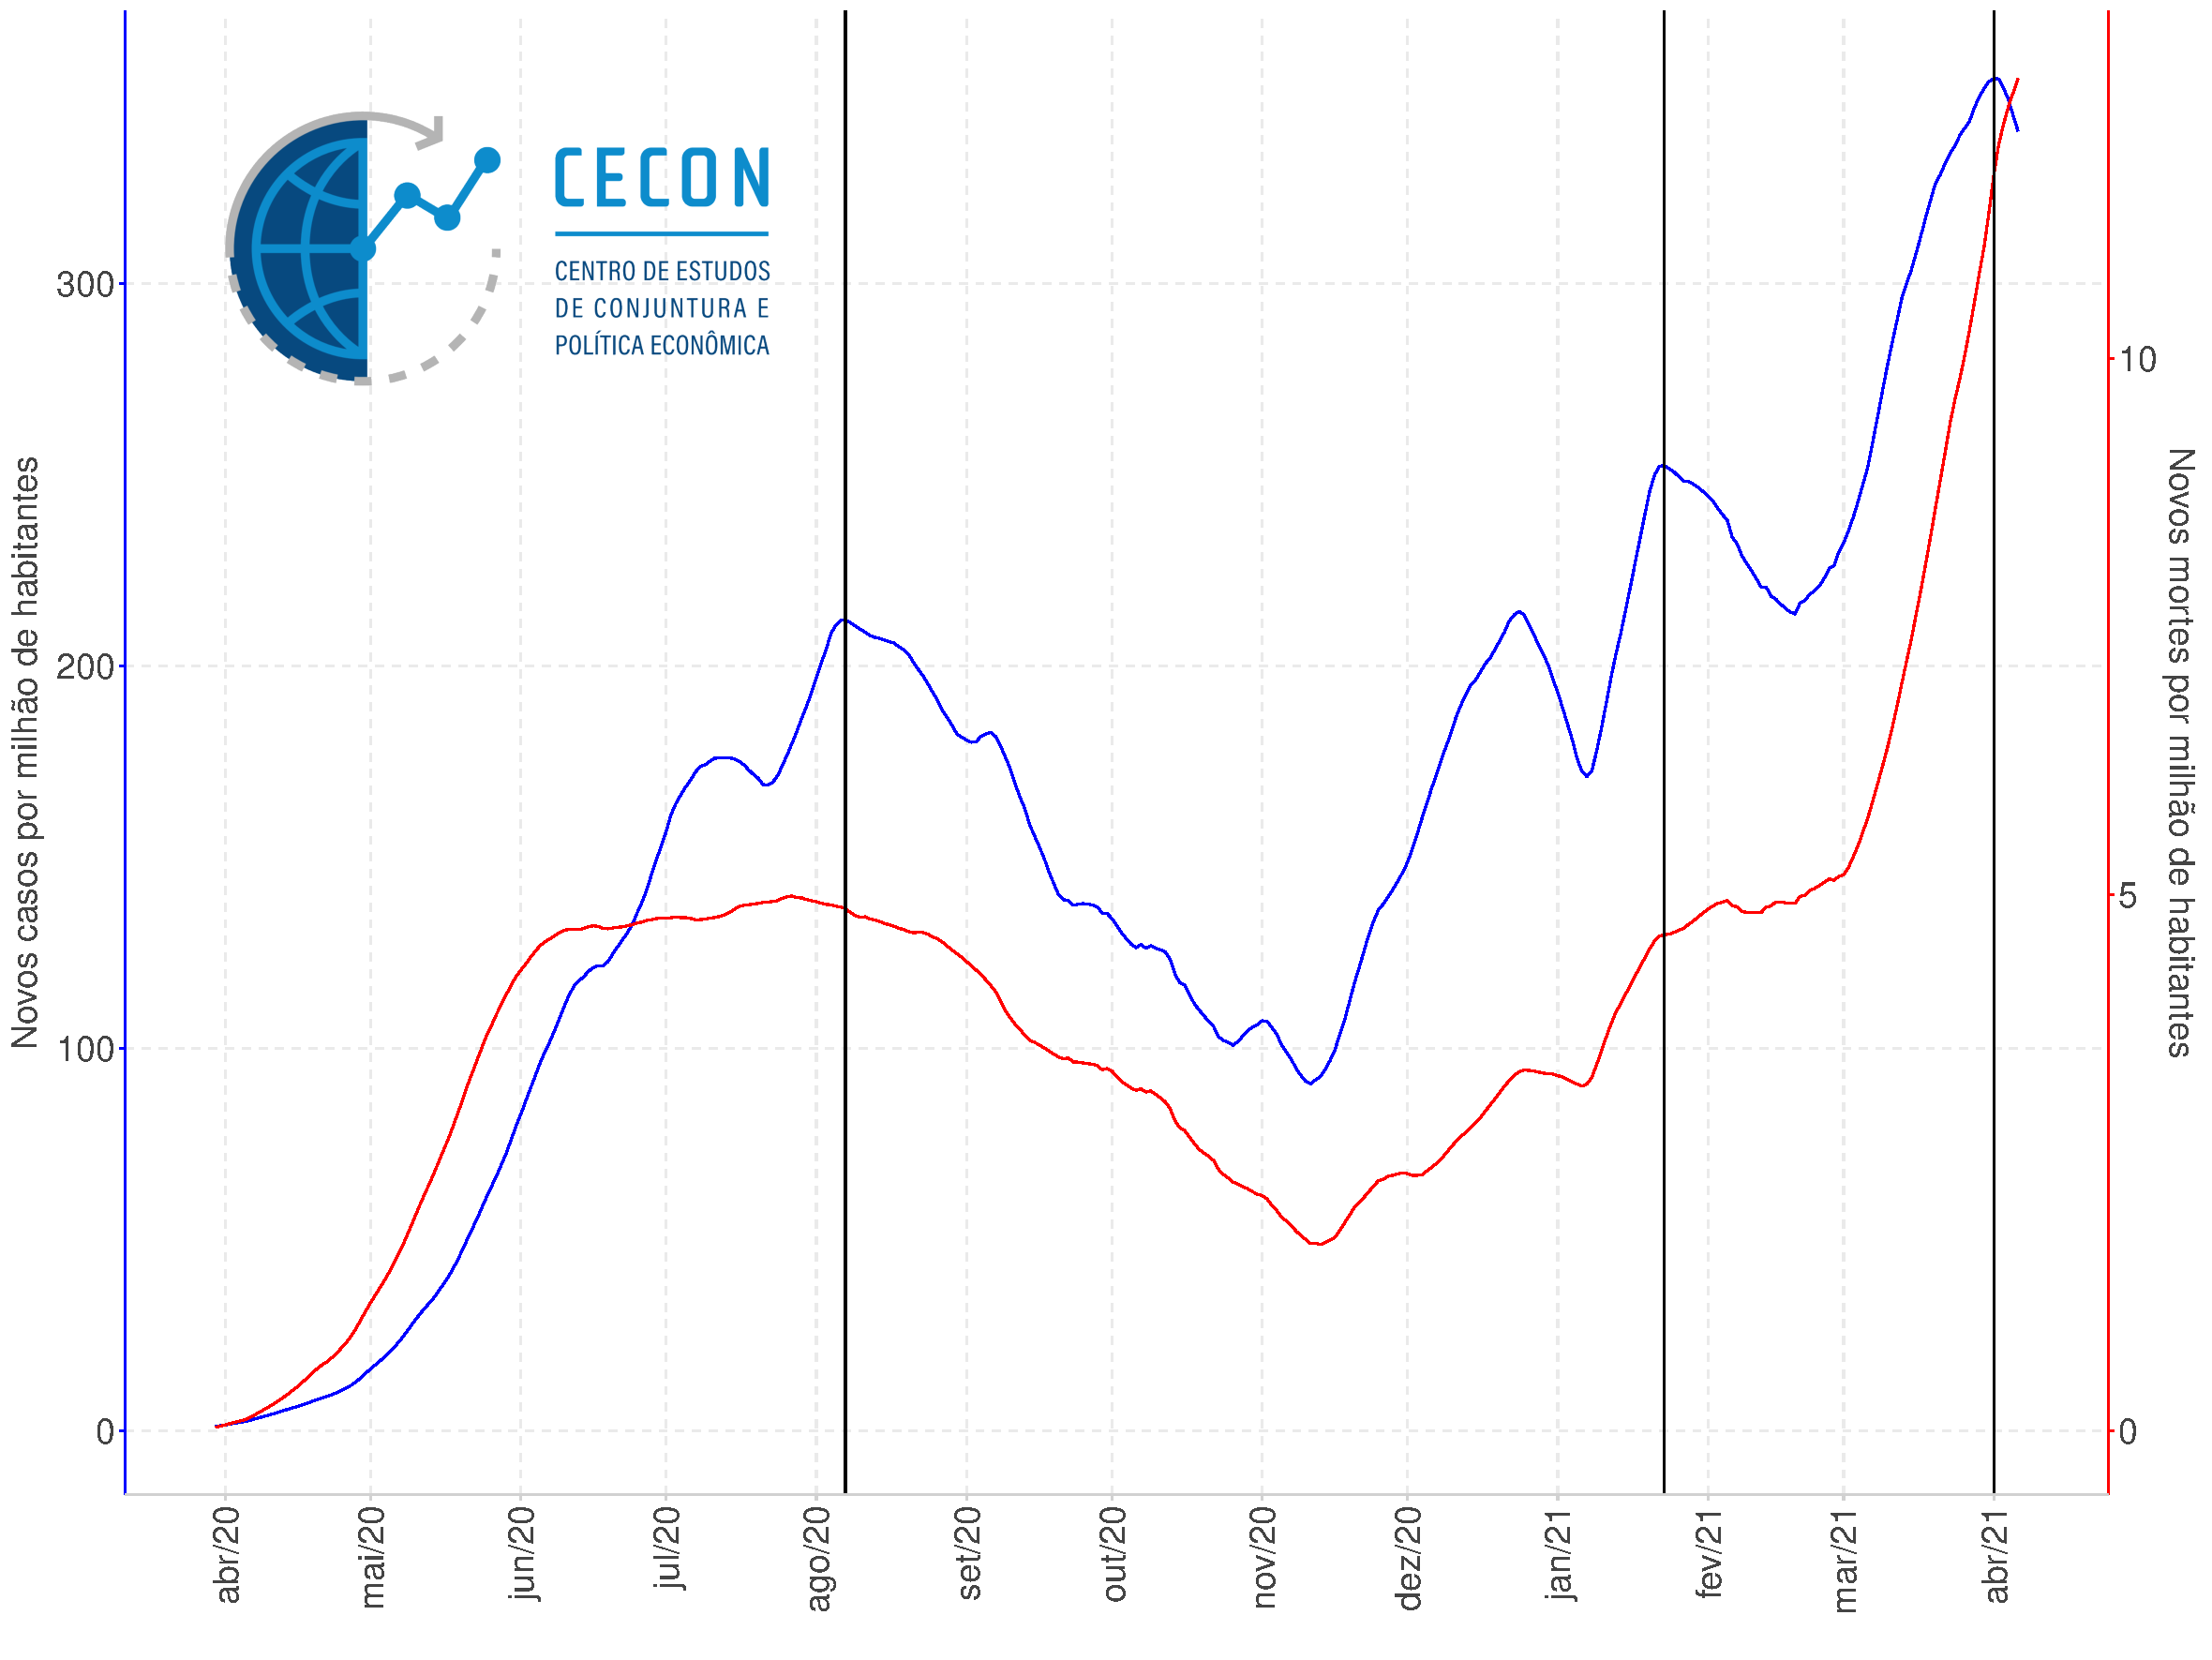
\includegraphics[width=.9\linewidth]{./figs/COVID/Estados/Brasil.pdf}
\end{figure}

\begin{figure}[htbp]
\caption{Novos casos a cada 1 milhão de habitantes (Mercosul + países selecionados, semana móvel)}
\centering
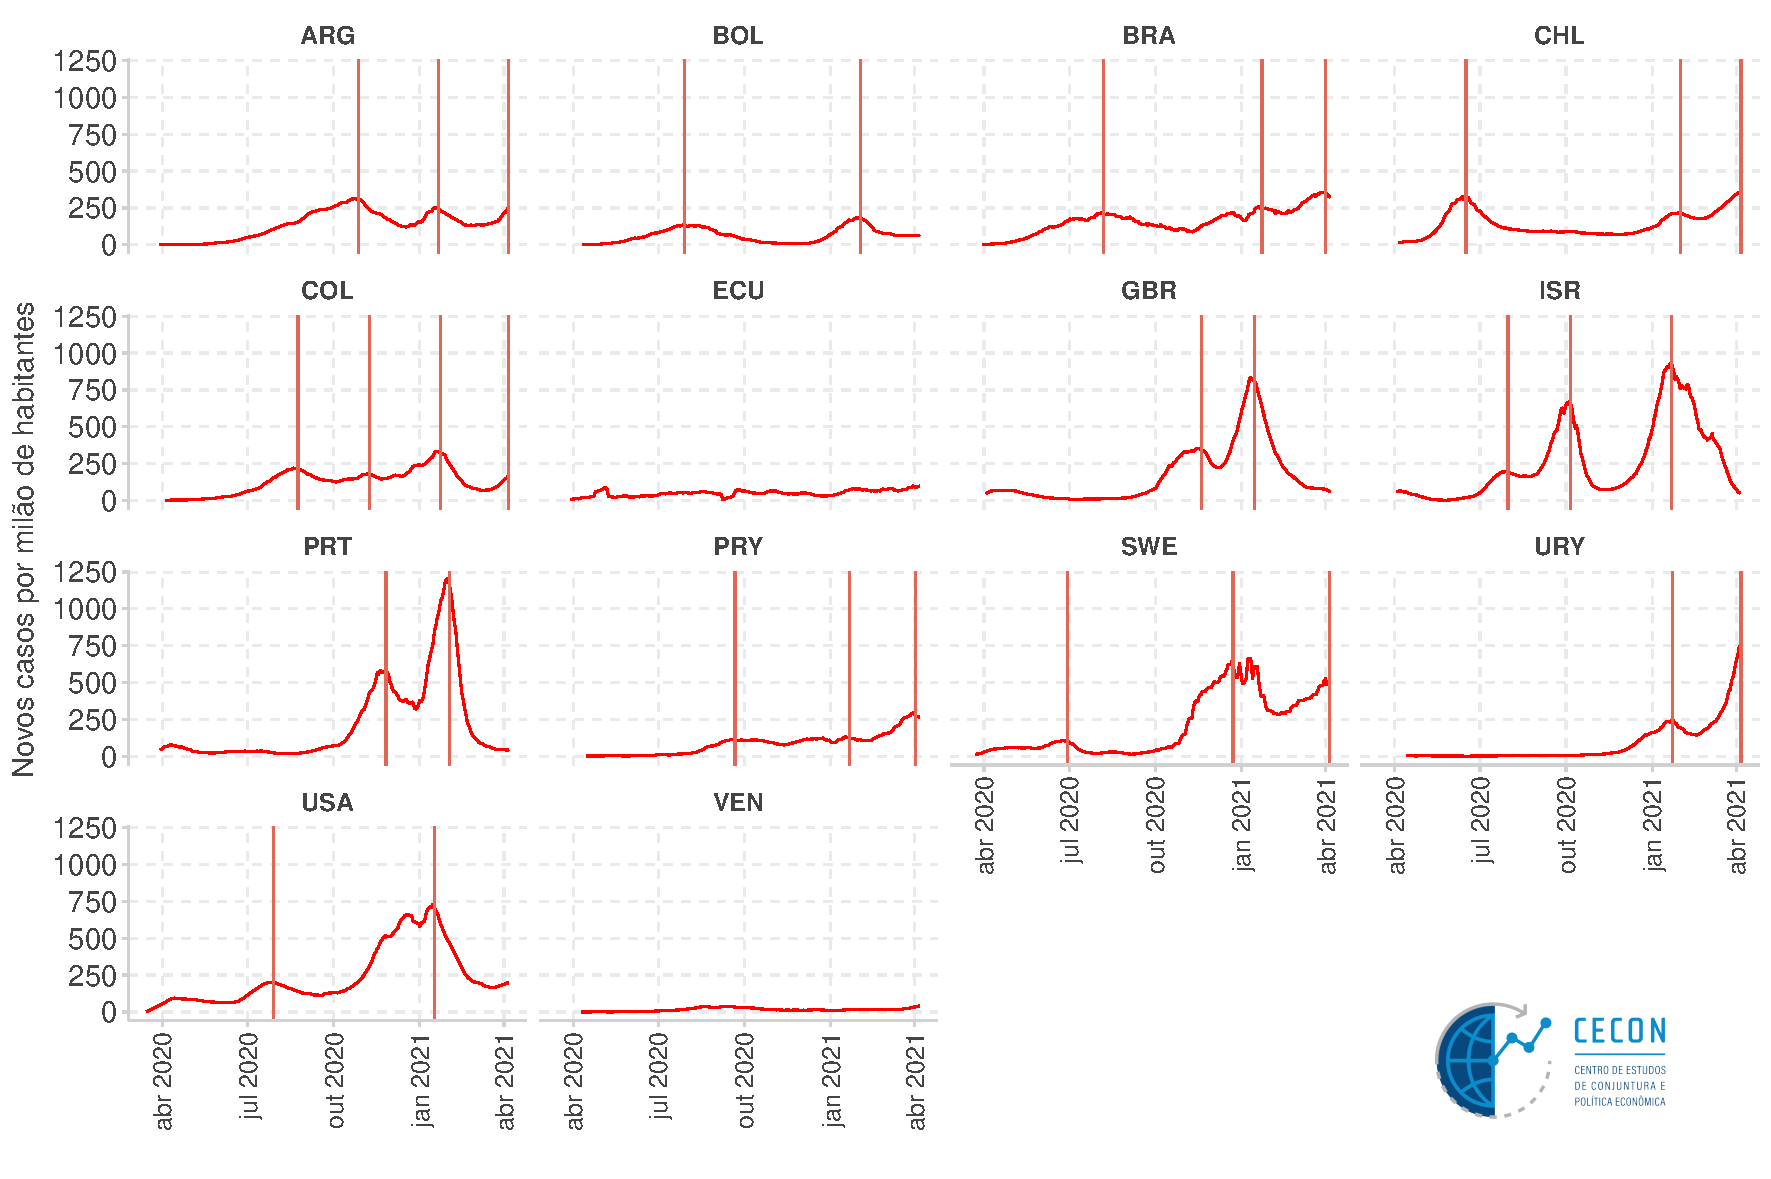
\includegraphics[width=.9\linewidth]{./figs/COVID/Picos.pdf}
\end{figure}

\begin{figure}[htbp]
\caption{Novos casos a cada 100 mil habitantes nos estados brasileiros (semana móvel)}
\centering
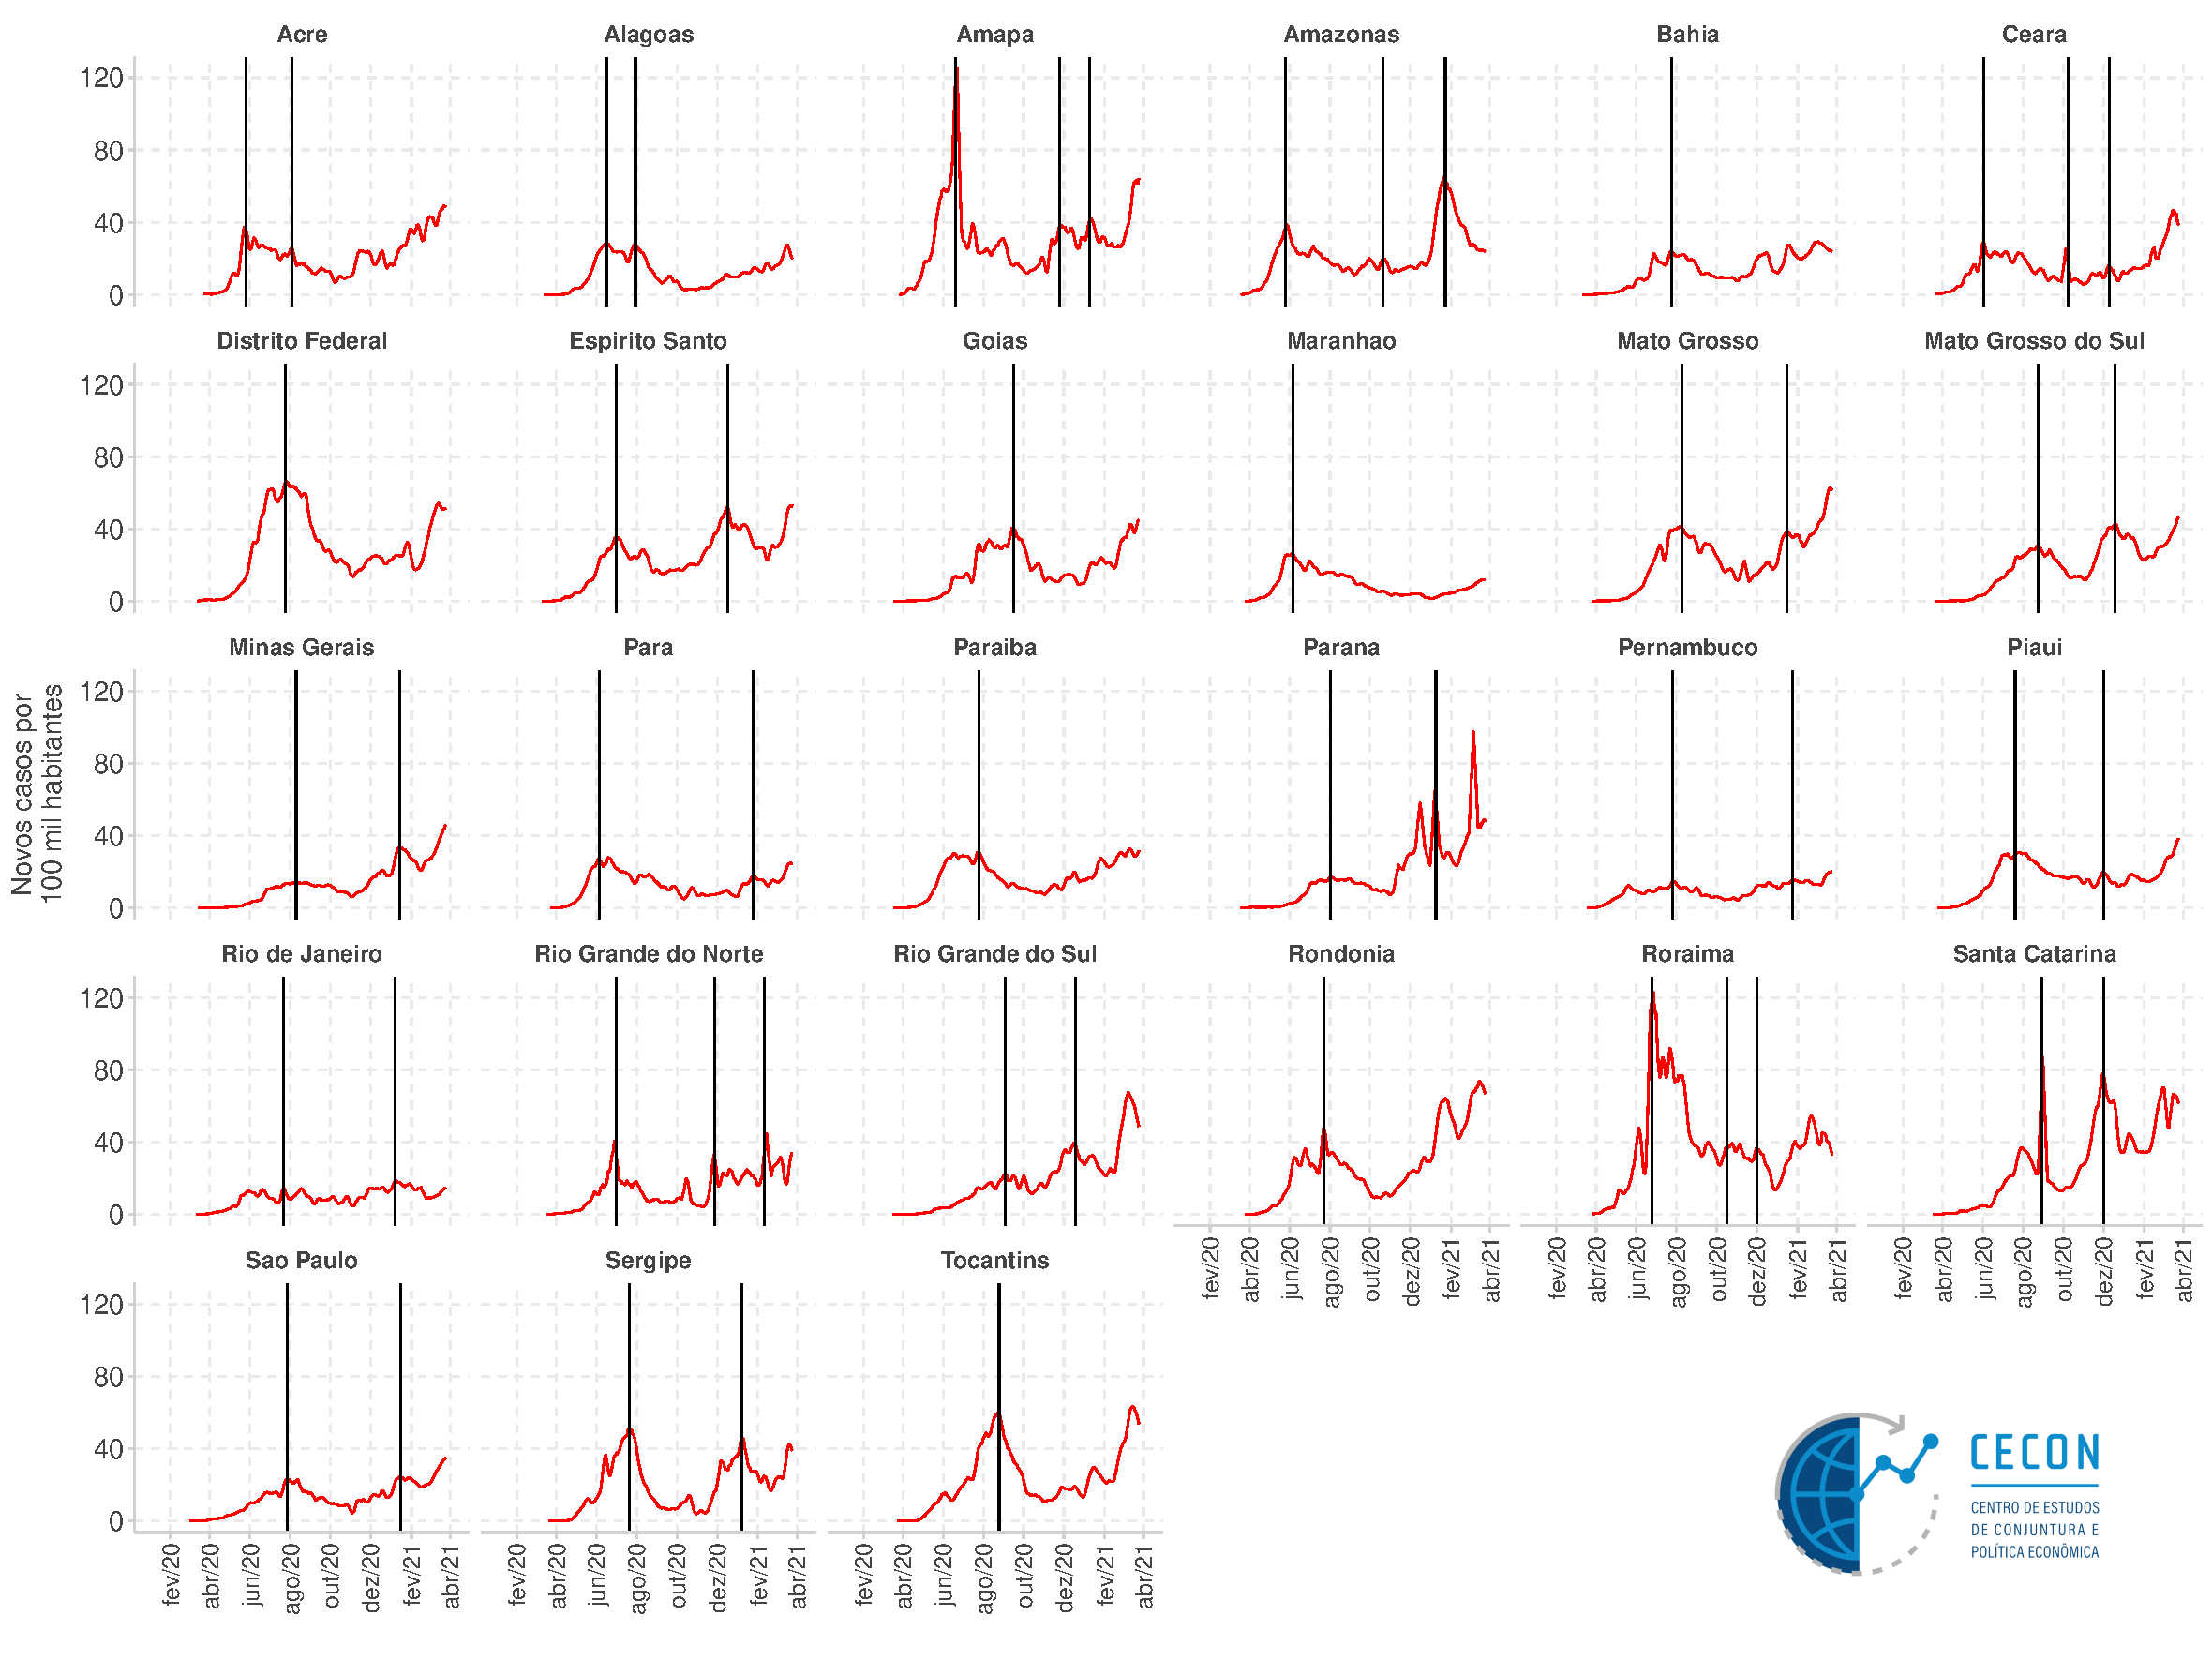
\includegraphics[width=.9\linewidth]{./figs/COVID/Estados/Casos.pdf}
\end{figure}

\begin{figure}[htbp]
\caption{Novas mortes a cada 100 mil habitantes nos estados brasileiros (quinzena móvel)}
\centering
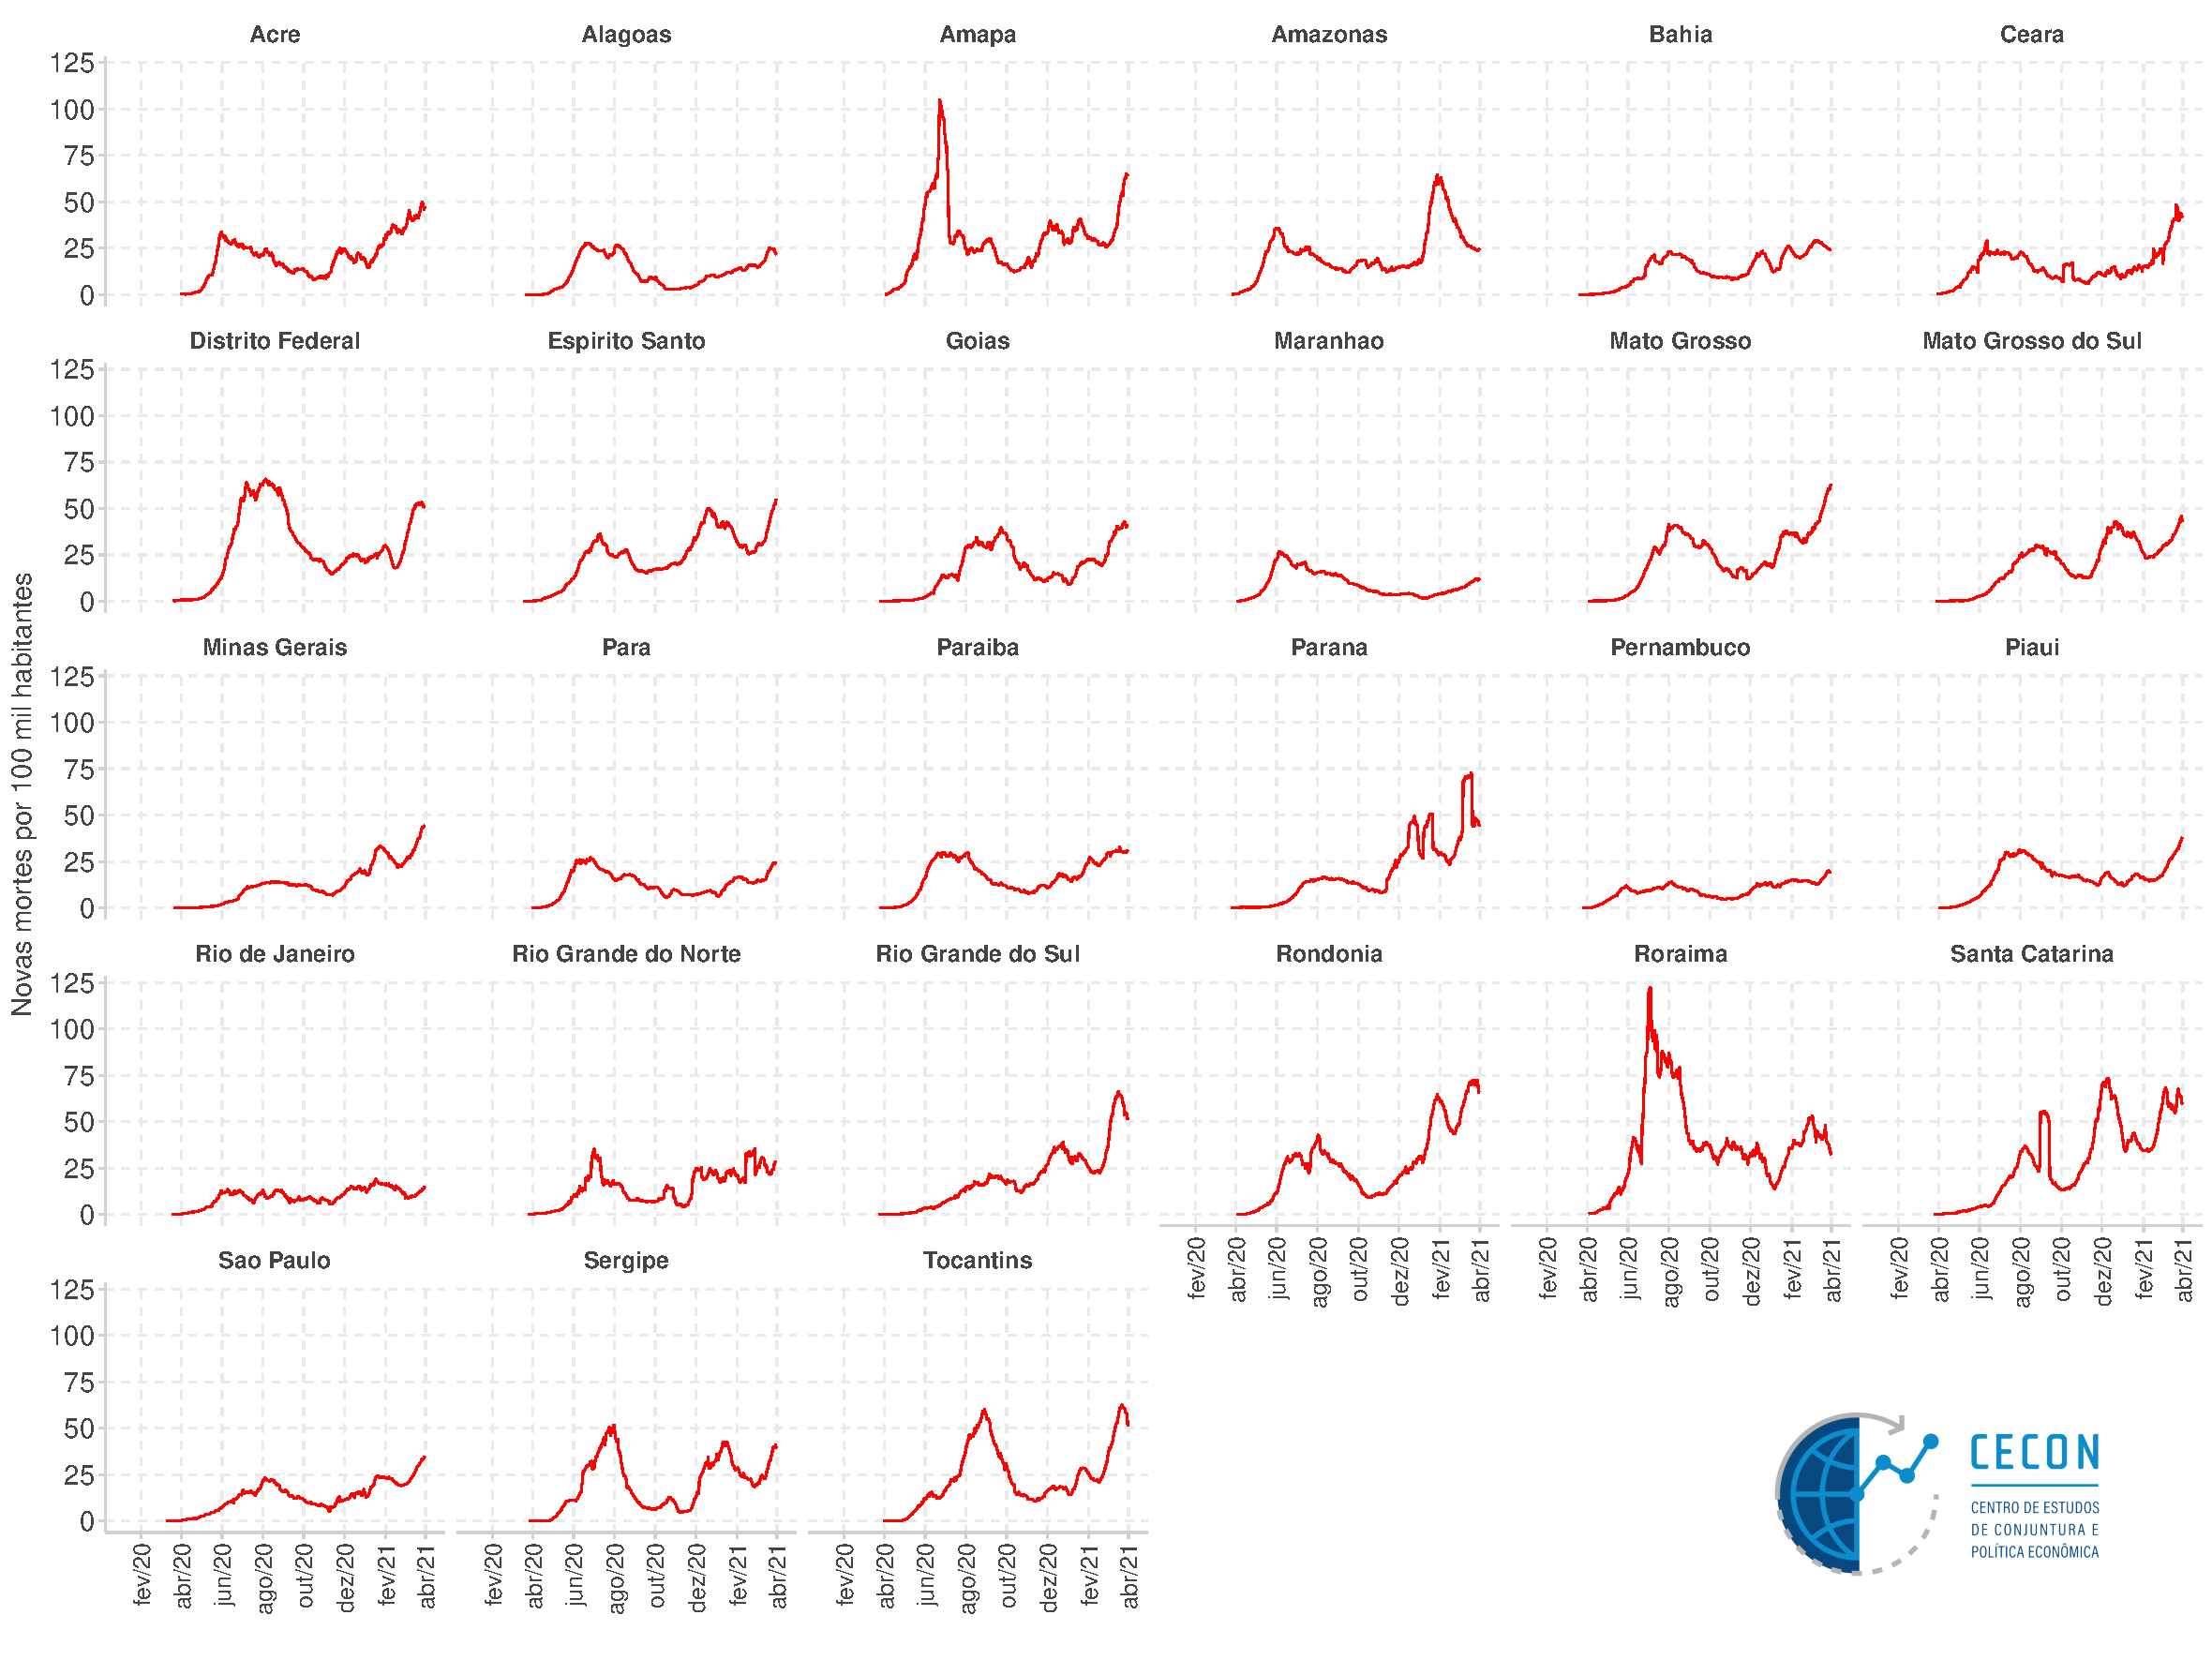
\includegraphics[width=.9\linewidth]{./figs/COVID/Estados/Mortes.pdf}
\end{figure}


\begin{figure}[htbp]
\caption{Pessoas em \emph{home office}}
\centering
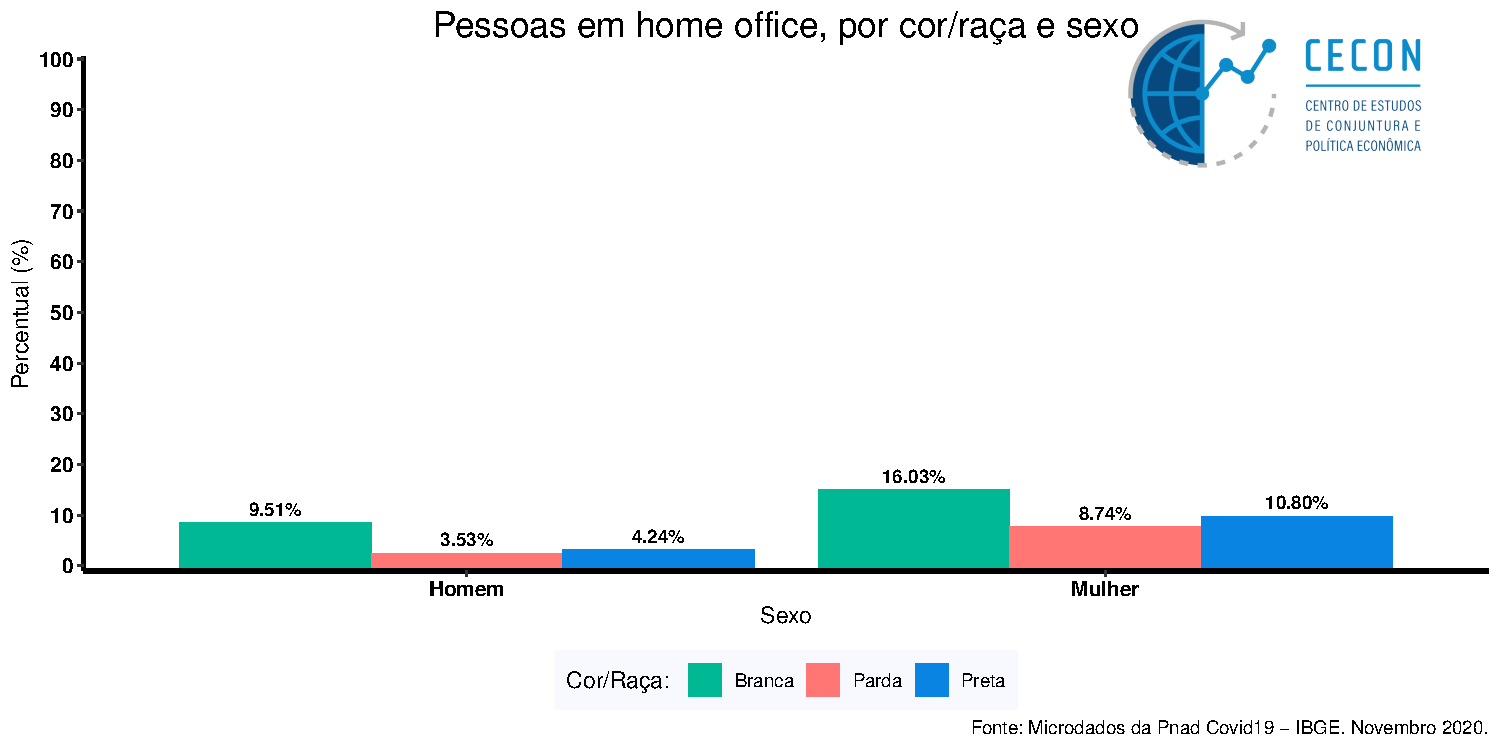
\includegraphics[width=.9\linewidth]{./figs/PNAD_COVID/home_sexo_cor.pdf}
\end{figure}
\end{document}
